\section{Concepción y Diseño}\label{section:design}

AutoETL se concibe como una herramienta para ser utilizada por los desarrolladores de almacenes de datos 
con el objetivo de aliviar la carga de trabajo en la implementación de los procesos de población de las 
estructuras analíticas. Su funcionamiento general consiste en generar las consultas y un pipeline que las utilice 
con el objetivo de poblar automáticamente un escenario analítico definido por el desarrollador. La 
figura \ref{fig:arquitectura} muestra los componentes de la aplicación, los cuales se corresponden 
con los componentes principales de una soluci\'on de ETL automático expuestos en el cap\'itulo \ref{chapter:auto-etl}.

\begin{figure}[H]
    \centering
    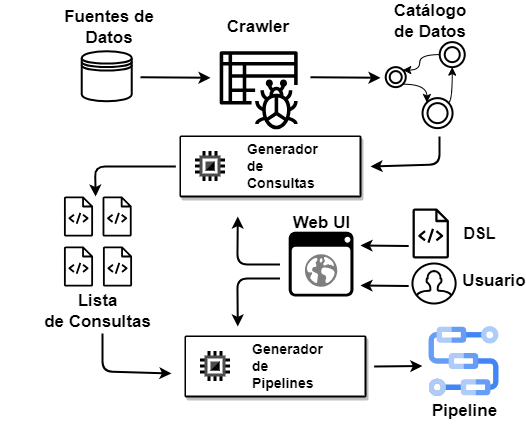
\includegraphics[width=0.60\textwidth]{Graphics/arch.drawio.png}
    \caption{Arquitectura del prototipo de AutoETL}
    \label{fig:arquitectura}
    \end{figure}



\begin{itemize}
    \item El primer elemento de la arquitectura propuesta son las \textbf{Fuentes de Datos}. En ellas yacen los 
        datos que poblar\'an el escenario analítico.
    \item La tarea del \textbf{Crawler} es explorar las fuentes de datos para recopilar información relevante sobre su estructura 
        con el fin de crear el \textbf{Catálogo de Datos} a partir de dicha información.
    \item El \textbf{Catálogo de Datos} es el repositorio que almacena metadatos sobre las fuentes de datos, los cuales son 
        utilizados en el proceso de la generación de consultas.
    \item El escenario analítico es definido mediante un script del lenguaje de dominio específico, dicho script debe ser programado por el desarrollador en 
        un editor de código de su preferencia. Los desarrolladores interactúan con la herramienta a través de una interfaz web, mediante la cual especifican el escenario 
        analítico a poblar, establecen conexiones con las fuentes de datos, consultan metadatos, configuran opciones necesarias 
        para el proceso de generación de consultas y del pipeline y finalmente ordenan la ejecución del pipeline generado. 
    \item El \textbf{Generador de Consultas} es el encargado de tomar la información proveniente del \textbf{Catálogo de Datos}, de la especificación
        del escenario analítico y de las configuraciones del usuario, para construir una lista de consultas, a partir de las cuales se creen y se pueblen 
        las estructuras de datos correspondientes al escenario analítico en cuestión.
    \item El \textbf{Generador de Pipelines} tiene la tarea de crear una secuencia lógica que define el flujo y el orden de ejecución de las actividades 
        que conforman el escenario de integración de datos, partiendo 
        de la lista de consultas generadas por el \textbf{Generador de Consultas} y de las especificaciones del usuario para la creación del pipeline. 
        Además, tiene la responsabilidad de ejecutar los pipelines, por tanto este componente es motor de integración de AutoETL.
    \item Por \'ultimo, el pipeline es una estructura en la que est\'a correctamente especificado el orden de ejecución de las consultas, 
        el método de carga y captura de los datos para la población, así como la frecuencia con que se se realizará la integración de los datos propiamente dicha.
\end{itemize}

En las secciones que aparecen a continuación se expone, de forma general, el funcionamiento de los módulos correspondientes a la primera 
aproximación de la solución propuesta y las principales consideraciones tomadas durante
su diseño.

\subsection{Crawler}

Este componente tiene la tarea de explorar las fuentes de datos para recopilar metadatos \'utiles para el proceso de generación
de consultas. Teniendo en cuenta que en esta primera aproximación se parte de fuentes relacionales, los metadatos extra\'idos son 
los nombres de las tablas de la base de datos fuente, por cada tabla se obtienen sus 
atributos, por cada atributo su tipo y si son llaves primarias. Además, por cada tabla se obtienen los atributos que son llaves 
for\'aneas y, por cada una, se extrae el nombre de la tabla a la que referencian y el atributo referenciado. Con esta información se construye 
el catálogo de datos.

\subsection{Catálogo de Datos}

Una vez que los metadatos de la fuente de datos son recopilados por el Crawler se pasa a poblar el Catálogo de Datos para dicha fuente. 
El Cat\'alogo de Datos se puebla, por cada fuente, 
con un pseudografo dirigido donde los nodos representan las tablas de la base de datos fuente y entre dos nodos $v$, $w$ 
existe un arco $<v,w>$ por cada llave for\'anea en $v$ que referencie a un atributo de $w$, en el caso de las relaciones unarias $v=w$. Cada nodo 
(tabla) guarda los nombres de los atributos de la tabla que representa, sus tipos y si son llaves primarias, for\'aneas o ambas. Cada arco $<v,w>$ 
guarda una tupla donde en la primera posición se encuentra el nombre del atributo de $v$ que es llave for\'anea y en la segunda 
posición el nombre del atributo de $w$ referenciado. Nótese que la dirección de un arco representa el sentido de la 
referencia de la llave for\'anea a la que representa como se muestra en la figura \ref{fig:datacatalogproposal}.

\begin{figure}[H]
    \centering
    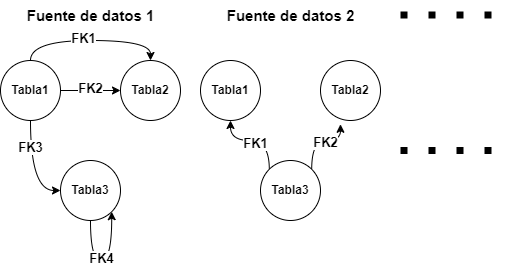
\includegraphics[width=0.5\textwidth]{Graphics/data_catalog.drawio.png}
    \caption{Estructura del catálogo de datos}
    \label{fig:datacatalogproposal}
\end{figure}

\subsection{Lenguaje de Dominio Espec\'ifico}

Como parte de los objetivos de la presente investigación est\'a la concepción y diseño de un lenguaje de dominio 
específico para la definición de escenarios analíticos. El objetivo del lenguaje es servir de vínculo 
entre el esquema relacional de la fuente de datos y el esquema dimensional del escenario analítico. El lenguaje 
brinda recursos sintácticos para la especificación de tablas de dimensiones y tablas de hechos, las cuales 
en su conjunto constituyen la definición de un esquema estrella.

La definición de atributos en las tablas de hechos o de dimensión constituye la base del vínculo entre 
los esquemas mencionados. La definición de un atributo 
implica detallar la procedencia y los valores que lo constituirán, es decir, la tabla de donde se extraerán los 
valores (el dónde). Asimismo, la definición de un atributo permite identificar el atributo concreto dentro de esa 
tabla cuyos valores se usarán para completar el atributo 
que estamos definiendo (el con qué). Este proceso garantiza que cada atributo se defina de manera clara y que 
se alimente correctamente con los datos pertinentes. De esta forma se entrelazan la representación relacional 
de la fuente de datos con el enfoque dimensional del esquema estrella. El listado de código \ref{code:CFG} presenta 
una primera aproximación de la gramática 
libre del contexto que da definición al DSL propuesto. Las palabras que comienzan con letra mayúscula indican no terminales y 
las palabras en minúscula indican terminales.

\begin{lstlisting}[label={code:CFG},caption={Gram\'atica libre del contexto del lenguaje de dominio espec\'ifico}]
    S' -> Dimensional_Schema
    Dimensional_Schema -> List_Dimensional_Tables
    List_Dimensional_Tables -> Dimensional_Table
                    | List_Dimensional_Tables Dimensional_Table

    Dimensional_Table -> dimension ID { List_Attr_Def }
                       | fact ID { List_Attr_Def }

    List_Attr_Def -> Attr_Def
                   | List_Attr_Def Attr_Def

    Attr_Def -> Attr_Expression Type Alias Level

    Attr_Expression -> T X
    X -> + T X | - T X | empty
    T -> F Y
    Y -> * F Y | / F Y | empty
    F -> Attr | number | (Attr_Expression)

    Attr -> Table : ID Modifier
          | Table : Func ( ID )
          | Table : sum ( ID )
          | Table : avg ( ID )
          | Table : count ( ID )
          | Table : max ( ID )
          | Table : min ( ID )

    Table -> ID | self

    Func -> weekday | monthstr

    Alias -> as ID | empty

    Level -> number | empty

    Type -> int | str | date | datetime | serial | float | numeric 
          | empty

    Modifier -> pk | fk to ID . ID | empty
\end{lstlisting}

Tal y como dicta la gramática, un esquema dimensional en forma de estrella (\textbf{Dimensional\_Schema}), 
en el contexto del DSL, est\'a compuesto por una lista de tablas 
dimensionales. 

Una lista de tablas dimensionales (\textbf{List\_Dimensional\_Tables}) est\'a compuesta por al menos 
una definición de tabla dimensional 
(\textbf{Dimensional\_Table}). 

Luego, la 
definición de una tabla dimensional (\textbf{Dimensional\_Table}) consta de la palabra clave \textbf{dimension} o \textbf{fact}, 
en caso de querer definir una dimension o una tabla de hechos respectivamente, un nombre para dicha tabla 
(\textbf{ID}), llaves con función delimitadora (\textbf{\{\}}) y dentro de estas una lista de definiciones de atributos
(\textbf{List\_Attr\_Def}). 

Una lista de definiciones de atributos est\'a compuesta por al menos una definición de atributo (\textbf{Attr\_Def}). 
La definición de un atributo consta de una expresión de atributos (\textbf{Attr\_Expression}), un tipo para el atributo 
definido, dicho tipo (\textbf{Type}) puede especificarse o no, un alias (\textbf{Alias}) que en caso de no ser vacío ser\'a el nombre del 
atributo en el esquema estrella y un nivel (\textbf{Level}) que es un entero que especifica la profundidad 
del atributo definido en la jerarquía de la dimensión. Una expresión de atributos (\textbf{Attr\_Expression}) no es m\'as que 
un recurso gramatical para expresar que una definición de atributo puede ser tanto un solo atributo (\textbf{Attr})
como una expresión aritmética en la que pueden participar atributos y n\'umeros. 

Un atributo (\textbf{Attr}) es la representación en el DSL de un atributo de la fuente de datos. Est\'a compuesto, 
fundamentalmente, 
por el nombre de la tabla de la fuente de datos (\textbf{Table}), dos puntos y el nombre del atributo de dicha tabla 
de donde se obtendrán los valores (\textbf{ID}). Además, puede contener especificaciones de modificadores (\textbf{Modifier}), 
los cuales pueden ser especificaciones de llave primaria o llave for\'anea. En esta primera versión del 
DSL un atributo puede ser llave primaria o llave for\'anea, pero no los dos a la vez. También, a los valores
extra\'idos del atributo con nombre (\textbf{ID}) y tabla (\textbf{Table}) se le puede aplicar funciones o agregaciones. Las 
funciones de agregación implementadas son suma (\textbf{sum}), promedio (\textbf{avg}), conteo (\textbf{count}), máximo (\textbf{max}) y 
mínimo (\textbf{min}). La palabra reservada \textbf{self} solo se debe usar para declarar la tabla en la definición de atributos 
que sean llaves primarias autogeneradas para las tablas de hechos.

Los tipos manejados por el lenguaje son genéricos y fácilmente mapeables con los tipos de los sistemas de 
gestión de bases de datos relacionales m\'as usados. El tipo \textbf{int} engloba a los n\'umeros enteros. 
Al tipo \textbf{str} pertenecen las cadenas de texto. Los tipos \textbf{date} y \textbf{datetime} agrupan a las fechas y a las fechas con 
hora respectivamente. El tipo \textbf{serial} se usa para las llaves primarias autogeneradas. El tipo \textbf{float} 
representa a los n\'umeros con coma flotante. Finalmente, al tipo \textbf{numeric} pertenecen todos los valores numéricos.

En caso de que una definición de un atributo solo contenga un atributo de una tabla de la fuente no es necesario 
especificar el tipo, pues el sistema automáticamente asignar\'a el tipo del atributo fuente al tipo del 
atributo que est\'a siendo definido. Sin embargo, si se define un atributo compuesto, es decir un atributo en 
cuya definición participe m\'as de un atributo de la fuente, es necesario precisar el tipo pues el sistema 
no es capaz de inferirlo.

Para especificar una llave for\'anea se deben escribir las palabras reservadas \textbf{fk} y \textbf{to} y luego puntualizar 
el nombre de una tabla del esquema estrella, un punto y el atributo referenciado.

Para asignar un alias a un atributo definido para una tabla del esquema dimensional se utiliza la 
palabra reservada \textbf{as} seguida del nombre del atributo.


\subsection{Generador de Consultas}

Este componente es el m\'as importante y el de mayor responsabilidad dentro de la arquitectura concebida, ya que es el 
encargado 
de generar el código SQL necesario para la creación y población del escenario analítico. Las consultas generadas 
se dividen en dos grupos: el grupo de creación de tablas y el grupo de selección de valores. El primer grupo 
está constituido por las consultas de creación de cada una de las tablas del esquema estrella. El segundo grupo 
consiste en las  consultas 
que permiten seleccionar los valores de los atributos necesarios para la población de una tabla del esquema estrella. 
Durante el proceso de construcción de las consultas de selección el generador de consultas infiere los joins 
necesarios para la concatenación apropiada de las tablas que intervienen en dichas consultas.

\subsubsection{Inferencia de joins}

En otras ocasiones, se ha enfrentado el problema de la inferencia de consultas utilizando representaciones
de bases de datos en forma de grafos y lenguajes 
de dominio específico. Entre estos trabajos se pueden mencionar aquellos que definen lenguajes de consulta 
conceptuales (\emph{Conceptual Query Languages}, CQL) que tratan de ocultar la complejidad de un esquema de bases de 
datos al vincular conceptos familiares para usuario con entidades presentes en la base de datos. Con este enfoque 
se puede citar el trabajo \cite{owei2001enriching} el cual propone
un algoritmo basado en caminos mínimos para encontrar el camino m\'as corto de joins que vincule los conceptos 
especificados, dando como resultado una sola interpretación de la consulta, lo cual no es factible 
puesto que lo ideal es analizar todas las posibles interpretaciones para una consulta y escoger la 
que sem\'anticamente responda a las necesidades del usuario. Otro enfoque para abordar el problema 
se refiere al uso de algoritmos de búsqueda de palabras clave (\emph{Keyword Search Algorithms}, KSA), específicamente  
aquellos que orientan la búsqueda sobre grafos. Si se representa un esquema de base de datos como un grafo
donde las tablas del esquema son los nodos y las relaciones entre las tablas son representadas mediante 
aristas, tomando los nombres de las tablas que intervienen en los joins de una determinada consulta de selección 
como las palabras clave a buscar en este grafo, se puede adaptar el problema de inferencia de joins 
a un problema de búsqueda de palabras clave. En este caso, la respuesta a la consulta de búsqueda 
es un sub\'arbol del grafo de búsqueda 
tal que, para toda palabra buscada, exista un nodo que la contenga. Recorriendo este sub\'arbol se puede construir 
f\'acilmente un join v\'alido para concatenar las tablas de una consulta de selección. Los trabajos 
\cite{kimelfeld2006finding,hristidis2003efficient,he2007blinks} exponen algoritmos eficientes para 
encontrar las $k$ mejores interpretaciones dado $k$, es decir, los $k$ mejores sub\'arboles que dan respuesta 
a la consulta de búsqueda. Sin embargo, la dependencia del parámetro $k$ para explorar todas las posibles 
interpretaciones,  
hizo que el autor se decantara por la propuesta de \cite{mason2005autojoin} para la resolución 
del problema de la inferencia de los joins planteado en los objetivos de la presente investigación.

El enfoque seleccionado parte de un grafo de joins, que no es m\'as que un grafo con las mismas características 
del Catálogo de Datos solo que empaca la información de los múltiples arcos que pueden existir entre 
dos nodos del catálogo en un \'unico arco y elimina los lazos (relaciones unarias), como muestra la 
figura \ref{fig:joingraphobtention}, pues estos \'ultimos no son 
relevantes dado que a partir de ellos solo se puede llegar al mismo nodo. Además, añade un arco $<v, w>$ si el nodo $v$ contiene un subconjunto 
de atributos contenidos en $w$ tal que todos los miembros de dicho subconjunto sean llaves for\'aneas en $v$
y sean llaves primarias en $w$. Nótese que estos subconjuntos de atributos cumplen con las restricciones 
de una llave for\'anea aunque la interrelación entre ambas tablas no aparezca explícitamente en la base de 
datos y, por tanto, representan un join válido.

\begin{figure}[H]
    \centering
    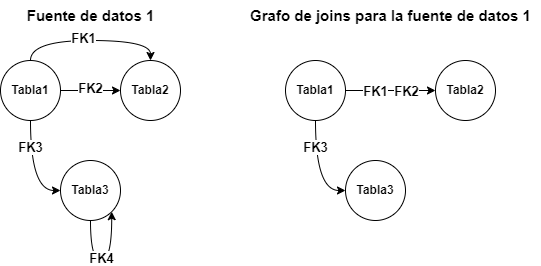
\includegraphics[width=0.60\textwidth]{Graphics/graph join transformation.drawio.png}
    \caption{Grafo de join asociado al pseudografo de una base de datos fuente.}
    \label{fig:joingraphobtention}
\end{figure}

Dado un conjunto de atributos fuente que conforman una tabla de dimensión o una tabla de hechos, el join necesario 
para concatenar apropiadamente estos atributos en una tabla \'unica es un sub\'arbol del grafo de joins. Pero, este join no tiene 
por qu\'e ser \'unico, pueden existir otros sub\'arboles que también constituyan joins válidos para lograr 
la la concatenación apropiada de los atributos. 

Explorar todos los posibles sub\'arboles durante una consulta sobre el grafo de joins mediante 
recorridos sucesivos es ineficiente. Para resolver este problema, \cite{mason2005autojoin} propone 
generar, a partir del grafo de joins, sub\'arboles maximales. Cada sub\'arbol maximal, al tener un juego 
de arcos diferentes, aporta potencialmente un join distinto. En el resto del documento estos sub\'arboles 
maximales ser\'an referidos como \'arboles de join. Una consulta sobre un determinado \'arbol de join no es m\'as que 
un conjunto de nodos (tablas) a concatenar mediante un join. Una respuesta a una consulta sobre un \'arbol de join es un sub\'arbol 
minimal que contenga los nodos de la consulta, es decir, el subárbol m\'as pequeño que contenga todos los nodos 
de la consulta, el cual constituye una interpretación 
de la consulta para dicho \'arbol de join.

Para computar los \'arboles de join, propuestas anteriores a \cite{mason2005autojoin} proponen hallar 
el subgrafo alcanzable desde un nodo y a este sub\'arbol calcularle todos los posibles \'arboles de 
expansión, los cuales constituyen los \'arboles de join. Repitiendo este proceso para 
cada nodo se logra 
calcular el conjunto de \'arboles de join, 
pero estos enfoques dan como resultado \'arboles de join duplicados y sobre todo 
es un algoritmo ineficiente y no computable para grafos de gran tamaño\cite{mason2005autojoin}.

El planteamiento de \cite{mason2005autojoin} introduce mejoras a este algoritmo. Establece que un \'arbol 
de join debe ser maximal, de no serlo, es posible que exista un \'arbol de join m\'as extenso que lo contenga. 
Tal \'arbol de join ampliado sería capaz de proporcionar, no solo 
las interpretaciones derivadas del \'arbol de join inferior en tamaño sino también adicionales, debido a que engloba 
un mayor número de nodos y, por ende, tiene la capacidad de brindar joins para consultas inaccesibles a su 
contraparte más limitada. Siguiendo esta idea, se propone solo computar el grafo alcanzable 
a los nodos del grafo de join que tengan grado interior (indegree) igual a cero o que est\'en en una 
componente fuertemente conexa en la que no existan arcos incidentes externos. 
Los \'arboles de join emanados de estos nodos raíz son inherentemente maximales, ya que la naturaleza de su raíz, 
implica que no hay otro subárbol que pueda subsumir los generados por dicha raíz.

Ahora, el conjunto de árboles de join puede ser precomputado, ya que depende únicamente del esquema de base de 
datos y no de las consultas. Esto traslada la computación más costosa fuera del tiempo de consulta. La cantidad
de \'arboles de join depende \'unicamente de la ambigüedad inherente al esquema de base de datos. Un esquema 
de base de datos no ambiguo resultar\'a en un único \'arbol de join y, por ende, en una \'unica interpretación 
para cada consulta. Las ambigüedades m\'as comunes se materializan en el grafo de join como nodos con m\'as de 
un arco incidente y como componentes fuertemente conexas.

\subsubsection{Fase de precomputaci\'on}

Dado un grafo de joins, la fase de precomputaci\'on se encarga de calcular los \'arboles de join. Como se expuso 
anteriormente, se identifican las posibles raíces y se halla el grafo alcanzable para cada una ellas. 
Por cada grafo alcanzable se computan sus \'arboles de expansión. El conjunto de todos los \'arboles en 
expansión calculados es el conjunto de \'arboles de join del grafo de join dado. Los \'arboles de join 
se almacenan y cuando se necesite responder una consulta son recuperados. El algoritmo recomendado en \cite{mason2005autojoin} 
para calcular 
los \'arboles de expansión (\emph{spanning trees}) de los grafos alcanzables es el propuesto por Harold N. Gabow y 
Eugene W. Myers en 1978 \cite{gabow1978finding}. El listado de código \ref{precom} muestra el pseudoc\'odigo 
del proceso de precomputaci\'on.

\begin{lstlisting}[label={precom}, caption={Pseudoc\'odigo del proceso de precomputaci\'on (tomado de \cite{mason2005autojoin})}]
    precomputation (JoinGraph dg)
    {
        allSCC = strongly connected components of dg
        rGraphs = empty
        for each scc in allSCC
            if (size scc == 1 and node has no in-edges)
                rGraphs = rGraphs + findReachable(n);
            else
                for each node n in scc
                    if (n has no in-edges from outside scc)
                        rGraphs = rGraphs + findReachable(n);
        joinTrees = empty
        for each reachable graph g in rGraphs
            joinTrees = joinTrees + findSpanningTrees(g)
        return joinTrees
    }
\end{lstlisting}

La demostración de correctitud de este algoritmo puede encontrarse en 
\cite{mason2005autojoin}. Con respecto a la complejidad temporal, el algoritmo de Harold N. Gabow y 
Eugene W. Myers tiene complejidad temporal $O(|V| + |E| + |E|N)$ donde $|V|, |E|, N$ son la cardinalidad 
del conjunto de vértices, la cardinalidad del conjunto de arcos y la cantidad de \'arboles de expansión respectivamente. 
Esta complejidad temporal, dentro del ciclo, es la que domina en el algoritmo. La cantidad de \'arboles de 
expansión de un grafo dirigido puede ser exponencial en el caso peor, caso en que el grafo de join sea 
completo; por tanto la complejidad temporal de este algoritmo en el caso peor es exponencial. Sin embargo, 
el caso peor, un esquema de bases de datos completamente conectado, no es com\'un. Además, la precomputaci\'on 
solo se realiza una vez, 
cuando se descubre el esquema de la base de datos, y solo se vuelve a realizar si dicho 
esquema sufre cambios en su definición.

\subsubsection{Fase de consulta}

Para dar respuesta a las consultas sobre los \'arboles de join, es decir, devolver un conjunto de joins que constituyen 
interpretaciones de la consulta, el procedimiento consiste en identificar los \'arboles de join que 
contengan todos los nodos (tablas) de la consulta. Luego, por cada \'arbol de join identificado, 
se busca el ancestro com\'un m\'as bajo (lowest common ancestor, LCA) de este conjunto de nodos. 
El sub\'arbol del \'arbol de join que da respuesta a la consulta y que constituye un join válido 
para la concatenación apropiada de las tablas, se forma mediante el enlace del LCA con los nodos requeridos 
mediante los caminos que los unen a ambos. El listado de código \ref{querytime} muestra el pseudoc\'odigo 
del algoritmo que computa la lista de joins asociados a una consulta.

\begin{lstlisting}[label={querytime}, caption={Pseudoc\'odigo del algoritmo de inferencia de joins}]
    get_joins (List_of_JoinTrees jts, List_of_Query_Tables query)
    {
        valid_join_trees = identify_join_trees(jts, query)
        all_joins = empty
        for each join_tree in valid_join_trees
            lca = lowest_common_ancestor(join_tree, query)
            join = reconstruct_sub_tree(join_tree, lca, query)
            all_joins = all_joins + join

        return all_joins
    }
\end{lstlisting}

La demostración de la correctitud del algoritmo \textbf{get\_joins} consiste en demostrar 
que todas las interpretaciones calculadas constituyen sub\'arboles minimales, que todas las interpretaciones calculadas
para una consulta pasada como argumento constituyen 
joins v\'alidos y que que el algoritmo devuelve todas las interpretaciones presentes en el grafo de join 
para la consulta pasada como argumento.

\begin{theorem}
    Todas las interpretaciones calculadas constituyen subárboles minimales.
\end{theorem}

Tomando al LCA entre los nodos de la consulta como raíz del subárbol que representa la interpretaci\'on, 
se asegura que no exista un nodo m\'as bajo a partir del cual se puedan alcanzar los nodos de la consulta. 
Cada nodo de la consulta se enlaza con el LCA mediante un camino simple, por tanto es de distancia m\'inima.
Luego no existe un subárbol m\'as pequeño que contenga los nodos de la consulta y por tanto es minimal. 


\begin{theorem}
    Todas las interpretaciones calculadas por el algoritmo \textbf{get\_joins} para una consulta pasada como 
    argumento constituyen joins v\'alidos.
\end{theorem}

Por la forma en que se construye el grafo de joins y los \'arboles de joins, el camino desde el 
LCA hasta un nodo de la consulta constituye una secuencia de joins v\'alidos sobre las llaves for\'aneas entre los 
nodos que participan en el camino. Luego las tablas resultantes de efectuar los joins que dictan los caminos 
desde el LCA hasta los nodos de la consulta se pueden concatenar mediante joins pues con que al menos una de ellas posea 
los atributos presentes en la tabla LCA es posible hacer join de esta tabla con el resto. Por tanto, el sub\'arbol que se forma por la union de los 
caminos desde el LCA hasta los nodos de la consulta representa una secuencia de joins v\'alida para concatenar 
apropiadamente las tablas representadas por nodos en la consulta pasada como argumento. 

\begin{theorem}
    El algoritmo \textbf{get\_joins} devuelve todas las interpretaciones presentes en el grafo de joins 
    para la consulta pasada como argumento.
\end{theorem}

Si existe una interpretaci\'on para una consulta que no es devuelta por el algoritmo entonces 
existe un sub\'arbol minimal $T$ del grafo de join que contiene todos los nodos de la consulta y que no est\'a contenido 
en ninguno de los \'arboles de join. Si la raíz de este sub\'arbol tiene indegree cero en el grafo de join entonces 
el algoritmo de precomputaci\'on debi\'o haber tomado en cuenta dicha ra\'iz para generar \'arboles de join, 
por tanto si existir\'ia un \'arbol de join que contiene al sub\'arbol $T$, contradicción. Si la ra\'iz $r$ del 
sub\'arbol $T$ no tiene indegree cero en el grafo de joins, se recorren sus ancestros, si algún ancestro $a$ tiene 
indegree cero entonces el algoritmo de precomputaci\'on produce \'arboles de join que contienen a $T$, lo 
cual es una contradicción; si ninguno de los ancestros de $r$ tiene indegree cero entonces existen 
ancestros de $r$ que pertenecen a componentes fuertemente conexas. Sea $a'$ un ancestro de $r$ que 
participa en una componente fuertemente conexa sin arcos incidentes exteriores a ella. El algoritmo 
de precomputaci\'on tiene en cuenta a $a'$ como ra\'iz para generar \'arboles de join y por tanto 
existe alguno que contiene a $T$, contradicción. Luego por reducci\'on al absurdo el algoritmo 
\textbf{get\_joins} devuelve todas las interpretaciones presentes en el grafo de join 
para la consulta pasada como argumento.

Luego, como se demostr\'o la veracidad de los tres teoremas anteriores se puede concluir que el 
algoritmo \textbf{get\_joins} es correcto.

Para el análisis de complejidad temporal se denota como $Q$ a la cantidad de tablas que contiene la consulta, 
$N$ a la cantidad de \'arboles de joins, $|V|$ a la cantidad de nodos del \'arbol de join m\'as extenso y $|E|$
a su cantidad de arcos. 

Calcular la intersección de dos conjuntos con $s$ y $t$ elementos respectivamente tiene 
complejidad temporal amortizada $O(s + t)$ si se utilizan conjuntos hash donde el costo de inserción y b\'usqueda 
tiene un una complejidad temporal amortizada de $O(1)$. Se añaden los $s$ elementos al conjunto hash en $O(1)$
y luego por cada uno de los $t$ elementos se pregunta si est\'an en el conjunto hash en $O(1)$, los elementos 
que se confirmen que est\'an en el conjunto hash conforman el conjunto intersección. Luego de estas aclaraciones 
se puede pasar al análisis de la complejidad temporal del algoritmo.

Para identificar cu\'ales \'arboles de join contienen todos los nodos de la consulta se puede implementar un índice 
inverso donde cada tabla (nodo) se enlaza a todos los árboles de join que contienen 
este nodo. La intersección de los conjuntos de árboles de join da como resultado todos los árboles de join 
que contienen todos los nodos especificados. Este procedimiento puede realizarse en $O(QN)$. 

El ancestro común más bajo (LCA) se computa hallando la intersección entre todos los ancestros de las tablas de la consulta y luego 
seleccionando el m\'as bajo en altura. Para una tabla (nodo) de la consulta hallar sus ancestros 
tiene complejidad $O(|V| + |E|)$ utilizando el algoritmo \emph{depth first search} (DFS) para recorrer el reverso de los arcos, 
este proceso se realiza $Q$ veces, una vez por cada nodo de la consulta. 

Hallar la intersección 
entre todos los ancestros de los nodos requeridos se realiza tomando un conjunto de ancestros 
como conjunto inicial y hallando la intersección de este conjunto con el resto de los conjuntos de ancestros, 
resultando al final en el conjunto de ancestros comunes. Este procedimiento tiene complejidad temporal 
$O(Q(|V| + |V|)) = O(Q(2|V|)) = O(Q|V|)$ asumiendo el caso peor que es que todos los conjuntos de ancestros 
tengan cardinalidad $|V|$. Luego de tener los ancestros comunes, se identifica el que posea menor altura 
en $O(|V|)$, resultando que el cómputo del LCA para un conjunto de nodos de tamaño $Q$ es $O(Q(|V| + |E|))$.

Reconstruir el sub\'arbol que se forma mediante el enlace de los caminos desde el LCA hasta los nodos 
de la consulta tiene complejidad temporal $O(|V| + |E|)$. Añadir elementos a una lista tiene complejidad 
$O(1)$ u $O(n)$, en dependencia de la implementación de lista que se utilice, siendo $n$ la cantidad 
de elementos de la lista, por simplicidad del análisis se toma como $O(1)$.

Finalmente, el algoritmo calcula los ancestros de los nodos de la consulta en $O(NQ)$. Luego por cada \'arbol de join realiza una búsqueda de LCA, 
una reconstrucción 
del sub\'arbol para ese LCA y se añade el sub\'arbol a una lista; efectuar estos tres pasos por cada \'arbol de join resulta en una complejidad temporal de 
$O(NQ(|V| + |E|))$. 
Por tanto, el algoritmo \textbf{get\_joins} tiene una complejidad 
temporal de $O(NQ + NQ(|V| + |E|)) = O(NQ(|V| + |E|))$.


\subsubsection{Fase de generaci\'on de c\'odigo}

El generador de consultas también tiene la tarea de producir el código SQL para la creación de las 
tablas del esquema estrella en el almacén de datos de destino y para la selección de 
los datos que alimentan el almacén desde la fuente. Para lograr este cometido se apoya 
en el algoritmo de inferencia de joins y en las especificaciones del escenario analítico 
mediante el lenguaje de dominio específico. Por tanto, para inferir las consultas para 
la creación y población de un escenario analítico es necesario que el desarrollador y 
usuario de la herramienta proporcione un script del DSL con la definición del escenario 
de inter\'es. Por cada tabla del esquema estrella se genera una consulta de creación y una 
consulta de selección.

Para construir la consulta de creación de una tabla del esquema estrella se recorre 
la lista definiciones de atributos que expone el script para dicha tabla y se agrega a la consulta 
su nombre, su tipo y su modificador. 
El nombre lo aporta el alias en el caso de atributos compuestos oo, en caso de ser un solo atributo y no tener un alias especificado, 
se mantiene el nombre que posee en la fuente de datos. Luego, se 
añaden las restricciones de llaves primarias y for\'aneas. Por \'ultimo, si se trata de una tabla 
de hechos, se añade una restricción de unicidad a la combinación de las llaves foráneas referidas a las 
tablas de dimensiones.

Para construir las consultas de selección de una tabla del esquema estrella se recorre la 
lista definiciones de atributos que expone el script para dicha tabla y se recolectan los 
nombres de las tablas de la fuente que intervienen en la definición, así como los 
nombres de los atributos requeridos para la población.
Se conforma una consulta de b\'usqueda con las tablas especificadas y se llama al algoritmo \textbf{get\_joins} (Listado de c\'odigo \ref{querytime}),
pasando como argumentos la consulta y la lista de \'arboles de joins precomputados para el esquema 
de base de datos de la fuente. As\'i se obtiene una lista de posibles joins para concatenar apropiadamente todas las 
tablas que intervienen en la consulta de selección.

En esta primera propuesta de la herramienta, el sistema no es capaz de inferir cu\'al es el join 
m\'as adecuado según las necesidades del usuario, dado que puede haber varios joins que resulten 
en la concatenación apropiada de las tablas especificadas, pero la semántica del resultado no tiene por qu\'e ser 
la misma. Por tanto, luego de obtener la lista de joins, el desarrollador debe seleccionar el que responda 
a sus intereses.

A partir del join seleccionado, se pasa a construir la consulta. En la cláusula \textbf{SELECT}, se 
incluyen todos los nombres de los atributos recopilados. Si se aplican funciones de agregación a ciertos 
atributos, se agrega la función específica junto con el atributo correspondiente como argumento. En la sección 
de la cláusula 
\textbf{FROM}, se coloca el join seleccionado. Si existen atributos recolectados cuyos valores a seleccionar 
son resultado de agregaciones,  se añade 
la cláusula \textbf{GROUP BY} con todos los atributos que intervienen en la cla\'usula \textbf{SELECT} a los que no 
se les aplique una función de agregación.


\subsection{Generador de Pipelines}

Luego de generar las consultas de creación y de selección, el usuario debe especificar 
mediante la interfaz gráfica el orden de ejecución de las consultas generadas, 
el tipo de extracción de datos de la fuente que utilizar\'a el pipeline, el tipo de carga 
en el sistema de destino y la frecuencia con que se ejecutar\'a. Con esta información y las 
consultas generadas se conforma un pipeline. 

Las consultas de creación son enviadas al sistema que albergar\'a el almacén de 
datos para su ejecución. Las consultas de selección se ejecutan en el sistema fuente de acuerdo al tipo 
de extracción especificado. Luego, el resultado es recibido por la herramienta y se pasa a generar una consulta 
de inserción para estos. Por \'ultimo, se ejecutan las inserciones de acuerdo al tipo de carga especificado.


Tras explorar detalladamente el proceso de concepción y diseño del marco de trabajo AutoETL y del 
lenguaje de dominio específico, el siguiente cap\'itulo se centra en la
implementaci\'on de cada uno de los componentes discutidos. Además, se detalla el proceso 
de experimentaci\'on realizado para comprobar el funcionamiento del prototipo implementado.
